\newpage
\section{Home Page}
Funkcjonalność ekranu początkowego aplikacji.
\begin{table}[H]
    \begin{center}
    \label{tab:table}
    \begin{tabularx}{1.1\textwidth} { 
    >{\raggedright\arraybackslash}X 
    | >{\raggedright\arraybackslash}X 
    | >{\raggedleft\arraybackslash}X}
    \textbf{Funkcja} & \textbf{Opis} & \textbf{Priorytet}\\
    \hline
    Dodaj&Pozwala dodać nową działkę&H\\
    \hline
    Wyszukaj&Mamy searchbar w którym możemy wyszukać działkę&H\\
    \hline
    Lista&Lista działek w której przewijamy istniejące działki i wybieramy po nazwie bądź obrazku&H\\
    \hline
    Wybierz&Panel podglądu i edycji istniejącej działki&H\\
    \hline
    Wyróżnione&Wyróżnienie działki&L\\
    \hline
    \end{tabularx}
    \end{center}
    \end{table}

\begin{figure}[htp]
    \centering
    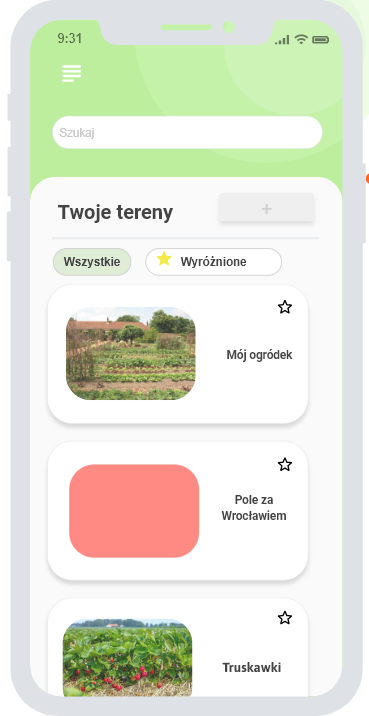
\includegraphics[width=5cm]{cibka.png}
\end{figure}